\documentclass[12pt,a4paper]{article}

\usepackage[UTF8]{ctex}
\usepackage[margin=2.2cm]{geometry}
\usepackage{amsmath,amssymb,amsthm,mathtools}
\usepackage{array}
\usepackage{booktabs}
\usepackage{enumitem}
\usepackage{xcolor}
\usepackage{graphicx}
\usepackage{fancyhdr}
\usepackage{fancyvrb}
\usepackage{lastpage}
\usepackage{hyperref}
\usepackage[most]{tcolorbox}
\usepackage{titlesec}
\usepackage{tabularx}
\usepackage{algorithm}
\usepackage{algpseudocode}
\usepackage{amsthm}
\usepackage{tikz}
\usetikzlibrary{arrows.meta}

\newtheorem{lemma}{引理}

\hypersetup{
  hidelinks
}

\definecolor{mainblue}{RGB}{34,72,112}
\definecolor{lightblue}{RGB}{241,246,252}
\definecolor{linegray}{RGB}{210,218,228}
\definecolor{textgray}{RGB}{90,98,108}

\setlength{\parindent}{2em}
\setlength{\parskip}{0.35em}
\setlength{\headheight}{25pt}
\linespread{1.2}

\pagestyle{fancy}
\fancyhf{}
\lhead{\textcolor{textgray}{\small 课程作业}}
\rhead{\textcolor{textgray}{\small \thepage/\pageref*{LastPage}}}
\cfoot{}
\renewcommand{\headrulewidth}{0.4pt}
\renewcommand{\headrule}{\hbox to\headwidth{\color{linegray}\leaders\hrule height \headrulewidth\hfill}}

\titleformat{\section}
  {\Large\bfseries\color{mainblue}}
  {\thesection}
  {0.6em}
  {}

\titleformat{\subsection}
  {\large\bfseries\color{mainblue}}
  {\thesubsection}
  {0.6em}
  {}

\titlespacing*{\section}{0pt}{1.2em}{0.6em}
\titlespacing*{\subsection}{0pt}{0.8em}{0.4em}

\newtcolorbox{infobox}{
  colback=lightblue,
  colframe=mainblue,
  boxrule=0.6pt,
  arc=2mm,
  left=1.2em,
  right=1.2em,
  top=0.8em,
  bottom=0.8em
}

\newtcolorbox{answerbox}{
  breakable,
  colback=white,
  colframe=linegray,
  boxrule=0.5pt,
  arc=2mm,
  left=1em,
  right=1em,
  top=0.8em,
  bottom=0.8em
}

\newtcolorbox{textbox}{
  breakable,
  colback=lightblue,
  colframe=linegray,
  boxrule=0.5pt,
  arc=1mm,
  left=1em,
  right=1em,
  top=0.6em,
  bottom=0.6em,
  before skip=0.8em,
  after skip=0.8em,
  fontupper=\small\ttfamily,
  before upper={\setlength{\parindent}{0pt}\raggedright}
}

\newenvironment{breakablealgorithm}[1]{%
  \par\addvspace{1em}
  \refstepcounter{algorithm}%
  \noindent\textbf{Algorithm~\thealgorithm. #1}\par\nobreak
  \noindent\rule{\linewidth}{0.4pt}\par\nobreak
  \vspace{0.4em}
}{%
  \par\vspace{0.2em}
  \noindent\rule{\linewidth}{0.4pt}
  \par\addvspace{1em}
}


\newcommand{\course}{算法设计与分析}
\newcommand{\homeworktitle}{第 8 次作业}
\newcommand{\studentname}{倪伟丰}
\newcommand{\studentid}{2024110089}
\newcommand{\classname}{24 大数据 2 班}
\newcommand{\teacher}{韩恺}
\newcommand{\duedate}{2026 年 5 月 27 日}

\begin{document}

\begin{center}
  {\Huge\bfseries\color{mainblue}\homeworktitle}\\[0.6em]
  {\Large\course}\\[1.2em]
  {\color{linegray}\rule{0.9\textwidth}{0.8pt}}
\end{center}

\begin{infobox}
\begin{tabularx}{\textwidth}{>{\bfseries}p{2.2cm} X >{\bfseries}p{2.2cm} X}
姓名 & \studentname & 学号 & \studentid \\
班级 & \classname & 教师 & \teacher \\
提交日期 & \duedate &  &  \\
\end{tabularx}
\end{infobox}

\section{Problem 1}

  The figure shows a flow network on which an $s$-$t$ flow has been computed. The capacity of each edge appears as a label next to the edge, and the numbers in boxes give the amount of flow sent on each edge. (Edges without boxed numbers have no flow being sent on them.)

  \begin{figure}[htbp]
    \centering
    
\includegraphics[width=0.86\textwidth]{1.png}
    \caption{Flow network for Problem 1.}
    \label{fig:problem1-flow-network}
  \end{figure}


    \begin{enumerate}[label=(\alph*), leftmargin=2.3em]
    \item (2 points) What is the value of the flow?

    \item (4 points) Is this a maximum flow in the graph? If so, identify a minimum $s$-$t$ cut and calculate its capacity; if not, write down an augmenting path in the residual graph, point out the bottleneck capacity on the path, and write down the flow resulted from augmenting along this path.

    To identify a cut, you may write down the nodes that are on the same side as the source $s$ in the cut. To identify an augmenting path in the residual graph, you do not need to draw the residual graph --- you may write down all the (directed) edges (e.g., $(b,d)$) in the path. Note that some edges in the residual graph may not be in the given graph. To write a flow, you need to write down the value of the flow along each edge in the given graph. E.g., in the current flow, $f((b,d))=8$.
  \end{enumerate}

\begin{answerbox}
\textbf{解答：}

\textbf{(a)} 该流的值为：

$$
v(f) = \sum_{e \text{out of } s} f(e) = 5+8 +5=18
$$

\textbf{(b)} 给出以下残差网络  $G_f$，其中包含以下正向边：

\[
\begin{aligned}
&s\to a:7,\quad a\to s:5,\quad b\to s:8,\quad c\to s:5,\quad b\to a:3,\\
&b\to d:4,\quad d\to b:8,\quad b\to c:5,\quad a\to d:3,\quad t\to a:5,\\
&c\to d:3,\quad c\to t:5,\quad t\to c:5,\quad t\to d:8.
\end{aligned}
\]

\begin{center}
\begin{tikzpicture}[
  >=Stealth,
  node/.style={circle,draw,fill=gray!18,minimum size=8mm,inner sep=0pt},
  edge/.style={->,thin,shorten >=1pt,shorten <=1pt},
  elab/.style={font=\scriptsize,fill=white,inner sep=1pt},
  every node/.style={font=\small}
]
  \node[node] (s) at (0,0) {$s$};
  \node[node] (b) at (2.25,0) {$b$};
  \node[node] (a) at (4.45,1.15) {$a$};
  \node[node] (c) at (4.45,-1.15) {$c$};
  \node[node] (d) at (6.75,0) {$d$};
  \node[node] (t) at (8.85,0) {$t$};

  \draw[edge] (s) to[bend left=10] node[elab,above,sloped,pos=.55] {7} (a);
  \draw[edge] (a) to[bend left=10] node[elab,below,sloped,pos=.55] {5} (s);
  \draw[edge] (b) -- node[elab,above,pos=.48] {8} (s);
  \draw[edge] (c) -- node[elab,below,sloped,pos=.50] {5} (s);

  \draw[edge] (b) -- node[elab,above,sloped,pos=.55] {3} (a);
  \draw[edge] (b) to[bend left=9] node[elab,above,pos=.50] {4} (d);
  \draw[edge] (d) to[bend left=9] node[elab,below,pos=.50] {8} (b);
  \draw[edge] (b) -- node[elab,below,sloped,pos=.47] {5} (c);

  \draw[edge] (a) -- node[elab,below,sloped,pos=.52] {3} (d);
  \draw[edge] (t) -- node[elab,above,sloped,pos=.50] {5} (a);

  \draw[edge] (c) -- node[elab,above,sloped,pos=.48] {3} (d);
  \draw[edge] (c) to[bend left=9] node[elab,below,sloped,pos=.50] {5} (t);
  \draw[edge] (t) to[bend left=9] node[elab,above,sloped,pos=.50] {5} (c);
  \draw[edge] (t) -- node[elab,above,pos=.50] {8} (d);
\end{tikzpicture}
\end{center}

因为在残量网络中存在增广路：
$$
s\to a\to d\to b\to c\to t.
$$
对应残量容量分别为：
$$
c_f(s,a)=7,
$$

$$
c_f(a,d)=3,
$$

$$
c_f(d,b)=8,
$$

$$
c_f(b,c)=5,
$$

$$
c_f(c,t)=5.
$$

所以该增广路的瓶颈容量为

\[
\min{7,3,8,5,5}=3.
\]

沿该路增广 (3) 单位后，流量变化如下：

\[
f(s,a):5\to 8,
\]
\[
f(a,d):0\to 3,
\]
\[
f(b,d):8\to 5
\]
\[
f(b,c):0\to 3,
\]
\[
f(c,t):5\to 8.
\]

增广后的流为：

\[
f(s,a)=8,\quad f(s,b)=8,\quad f(s,c)=5,
\]

\[
f(b,a)=0,\quad f(b,d)=5,\quad f(b,c)=3,
\]

\[
f(a,d)=3,\quad f(a,t)=5,
\]

\[
f(c,d)=0,\quad f(c,t)=8,\quad f(d,t)=8.
\]

新的流值为

\[
18+3=\boxed{21}.
\]

\end{answerbox}

\section{problem 2}

  We are given a flow network $G=(V,E)$ and labels $f:E\to \mathbb{R}_+$.


\subsection{}

 Give an algorithm that verifies whether $f$ is a maximum flow. Your algorithm needs to run in linear time, i.e. in time $O(|V|+|E|)$.

\begin{answerbox}
\textbf{解答：}

给定流网络 $G=(V,E)$、容量函数 $c:E\to \mathbb{R}_+$ 以及边标签 $f:E\to \mathbb{R}_+$。

\textbf{首先检查 $f$ 是否为合法流。}

对每条边 $e\in E$，检查容量约束
\[
  0\le f(e)\le c(e).
\]
然后对每个点 $v\in V$ 维护一个净流入量数组 $b(v)$，初始化为
\[
  b(v)=0,\qquad \forall v\in V.
\]
对每条边 $e=(u,v)$，执行
\[
  b(u)\leftarrow b(u)-f(e),\qquad b(v)\leftarrow b(v)+f(e).
\]
最后检查所有中间点 $v\in V\setminus\{s,t\}$ 是否满足
\[
  b(v)=0.
\]
若容量约束或流量守恒不成立，则 $f$ 不是最大流。

\textbf{构造残量网络并检查增广路。}

如果 $f$ 是合法流，则构造残量网络 $G_f$。对每条原边 $e=(u,v)$：
\begin{itemize}[leftmargin=2em]
  \item 若 $c(e)-f(e)>0$，则在残量网络中加入正向边 $(u,v)$；
  \item 若 $f(e)>0$，则在残量网络中加入反向边 $(v,u)$。
\end{itemize}
然后在残量网络 $G_f$ 中从 $s$ 出发进行一次 BFS 或 DFS。若能够到达 $t$，说明存在增广路，因此 $f$ 不是最大流；若不能到达 $t$，则 $f$ 是最大流。

\textbf{正确性证明。}

如果第一步检查失败，则 $f$ 不是合法流，自然不可能是最大流。

如果第一步检查通过，则 $f$ 是合法流。根据最大流增广路定理，一个合法流是最大流，当且仅当它的残量网络中不存在从 $s$ 到 $t$ 的增广路。算法第二步正是通过一次 BFS 或 DFS 判断残量网络中是否存在 $s$ 到 $t$ 的路径。因此算法的判断是正确的。

\textbf{运行时间分析。}

检查容量约束和流量守恒只需扫描所有边一次，时间为 $O(|V|+|E|)$。构造残量网络也只需扫描所有边一次，时间为 $O(|E|)$。最后一次 BFS 或 DFS 的时间为 $O(|V|+|E|)$。因此总运行时间为
\[
  O(|V|+|E|).
\]

\end{answerbox}

\subsection{}

 Suppose we have verified that $f$ is indeed a maximum flow. Further assume that all capacities in $G$ are integers, and $f$ is integer-valued as well. Also, there is no cycle in $G$ such that $f$ is positive on each edge of the cycle. Now take an edge $e^*$ from $E$ with $c_{e^*}>0$, and reduce its capacity by one unit. Give a linear-time algorithm that finds a maximum flow in the resulting network.

\begin{answerbox}
\textbf{解答：}

设被减少容量的边为
\[
  e^*=(u,v).
\]
原容量为 $c(e^*)$，减少后的容量为
\[
  c'(e^*)=c(e^*)-1.
\]
设原最大流 $f$ 的流值为 $F$。

\textbf{算法描述}

分两种情况讨论：

\textbf{情况一：}若
\[
  f(e^*)\le c(e^*)-1,
\]
则容量减少后，原流 $f$ 仍满足所有容量约束，所以 $f$ 仍是新网络中的一个可行流。由于减少容量不会使最大流值变大，而原网络中最大流值为 $F$，所以新网络中的最大流值仍为 $F$。此时直接输出原流 $f$。

\textbf{情况二：}若
\[
  f(e^*)=c(e^*),
\]
则容量减少后，原流在边 $e^*$ 上违反容量约束 $1$ 个单位。

考虑由所有正流边构成的子图
\[
  H=(V,E_H),\qquad E_H=\{e\in E:f(e)>0\}.
\]
题目假设不存在一个有向环使得环上每条边的流量都为正。因此，在正流子图 $H$ 中，边 $e^*$ 位于某条正流的 $s$-$t$ 路径上。于是可以在 $H$ 中找到一条路径
\[
  P:s\leadsto u\to v\leadsto t
\]
使得路径 $P$ 上每条边的流量都为正。

沿路径 $P$ 上的每条边都将流量减少 $1$，得到一个新流 $f_1$。因为路径上每条边原本都有正整数流量，所以减少 $1$ 后仍然非负。并且边 $e^*$ 的流量也被减少 $1$，从而满足新的容量约束。此时 $f_1$ 是新网络中的一个可行流，且流值为
\[
  F-1.
\]

接下来，在新网络和流 $f_1$ 的残量网络中，从 $s$ 出发做一次 BFS 或 DFS。

若不能到达 $t$，则不存在增广路，由最大流增广路定理可知 $f_1$ 已经是新网络的最大流。

若能够到达 $t$，则沿找到的增广路增广 $1$ 单位，得到一个流值为 $F$ 的可行流。由于新网络的容量只比旧网络少了 $1$，其最大流值不可能超过旧网络的最大流值 $F$，所以这个流值为 $F$ 的流一定是新网络的最大流。

\textbf{正确性证明}

如果 $f(e^*)\le c(e^*)-1$，则容量减少后原流仍可行。新网络的可行流集合是原网络可行流集合的子集，因此新网络最大流值不超过 $F$。但原流 $f$ 在新网络中仍可行且流值为 $F$，所以它仍是最大流。

如果 $f(e^*)=c(e^*)$，则必须降低经过 $e^*$ 的流量。由题目给出的正流无环条件，正流可以视为若干条 $s$-$t$ 正流路径的叠加，且边 $e^*$ 位于其中某条正流路径上。因此沿包含 $e^*$ 的正流路径整体减少 $1$，可以保持所有中间点的流量守恒，并得到流值为 $F-1$ 的可行流 $f_1$。

在容量只减少 $1$ 的情况下，新最大流值最多比原最大流值少 $1$，所以新最大流值只可能是 $F$ 或 $F-1$。算法随后在 $f_1$ 的残量网络中寻找增广路：若存在增广路，则增广后流值回到 $F$，必为最大流；若不存在增广路，则根据最大流增广路定理，$f_1$ 本身就是最大流。

\textbf{运行时间分析}

判断是否仍可行只需检查边 $e^*$，时间为 $O(1)$。在正流子图中寻找包含 $e^*$ 的正流 $s$-$t$ 路径，可以通过一次线性时间搜索完成。调整路径上的流量需要的时间不超过路径长度，因此为 $O(|V|)$。最后构造并搜索残量网络的时间为 $O(|V|+|E|)$。所以总运行时间为
\[
  O(|V|+|E|).
\]

\end{answerbox}

\section{Problem 3}

(For this problem, you do not need to give proofs of correctness for your algorithms, but you should analyze their running time.) You are helping a company set up its customer service ``intelligently''. The company collects data about the customers' background and special needs, and identify customer service representatives that can serve them better. In particular, for each of its $n$ customers online, we are given a subset of the $n$ representatives who are deemed qualified to serve that customer (that is, different customers have different subsets of representatives that serve them well). Each customer needs one representative to serve him/her, and each representative can serve at most one customer at a time.

\subsection{}

 (5 points) Given this information, give an algorithm that decides whether all the customers can be served simultaneously, each by a representative qualified to serve him/her. If this is possible, your algorithm should also assign each customer a qualified representative. Your algorithm should run in time $O(n^3)$.

\begin{answerbox}
\textbf{解答：}

\textbf{算法。}

构造如下流网络。加入源点 $s$ 和汇点 $t$。对每个客户 $c_i$，加入边$(s,c_i)$，容量为 $1$。

如果代表 $r_j$ 有资格服务客户 $c_i$，则加入边$(c_i,r_j)$，容量为 $1$。

对每个代表 $r_j$，加入边$(r_j,t)$，容量为 $1$。

然后在该网络上求最大流。

若最大流值为 $n$，则说明所有客户都可以被同时服务。此时，对每条满足
\[
  f(c_i,r_j)=1
\]
的边 $(c_i,r_j)$，安排代表 $r_j$ 服务客户 $c_i$。

若最大流值小于 $n$，则说明不存在一种安排能够使所有客户同时被服务。

\textbf{运行时间分析}

该网络共有$2n+2$个点。边数最多为$n+n+n^2=O(n^2)$。因为所有容量均为整数且最大流值至多为 $n$，使用 Ford-Fulkerson 算法时，每次增广至少使流值增加 $1$，所以最多进行 $n$ 次增广。每次寻找增广路需要 $O(n^2)$ 时间。因此总运行时间为
\[
  O(n\cdot n^2)=O(n^3).
\]

\end{answerbox}

\subsection{}

 (8 points) Suppose you succeed in part (a), and your algorithm finds a way to serve all customers simultaneously. It turns out there is a VIP customer who is demanding but unpredictable. The company would like to give this customer the privilege to choose a representative, but worries that this may affect its capacity to serve the other customers. Give an algorithm that decides, for each of the $n$ representatives, whether it is possible to let that representative serve the VIP customer while the other $n-1$ customers can all be served by qualified representatives. Your algorithm should run in time $O(n^3)$.

\begin{answerbox}
\textbf{解答：}

假设 VIP 客户为 $c_1$。由第 (a) 问，已经得到一个完美匹配 $M$，即每个客户都被分配给一个有资格服务他的代表，且每个代表至多服务一个客户。

现在需要对每个代表 $r\in R$ 判断：是否存在一个完美匹配 $M'$，使得 VIP 客户 $c_1$ 被分配给代表 $r$。


\textbf{算法描述}

构造一个有向图 $D$，其点集为
\[
  C\cup R.
\]
对每条合格边 $(c_i,r_j)$：
\begin{itemize}[leftmargin=2em]
  \item 如果 $(c_i,r_j)\in M$，则在 $D$ 中加入有向边
  \[
    r_j\to c_i;
  \]
  \item 如果 $(c_i,r_j)\notin M$，则在 $D$ 中加入有向边
  \[
    c_i\to r_j.
  \]
\end{itemize}
然后对有向图 $D$ 求强连通分量。

对每个代表 $r\in R$，按照如下规则判断：
\begin{itemize}[leftmargin=2em]
  \item 如果 $(c_1,r)$ 不是合格边，则答案为 No；
  \item 如果 $(c_1,r)\in M$，则答案为 Yes；
  \item 如果 $(c_1,r)\notin M$，则检查 $c_1$ 与 $r$ 是否在同一个强连通分量中。若在同一个强连通分量中，则答案为 Yes；否则答案为 No。
\end{itemize}


\textbf{算法解释}

匹配边和非匹配边交替出现的结构称为交替结构。在上述有向图 $D$ 中，非匹配边按照客户到代表的方向定向，匹配边按照代表到客户的方向定向。因此，$D$ 中的有向路径正好对应二分图中的交替路径。

如果 $(c_1,r)$ 本来就在当前匹配 $M$ 中，则当前匹配已经满足要求。

如果 $(c_1,r)$ 不是当前匹配边但它是一条合格边，那么要让 $r$ 服务 VIP，就需要把边 $(c_1,r)$ 加入匹配，并沿某个交替环调整匹配。这个交替环包含非匹配边 $(c_1,r)$。在有向图 $D$ 中，这等价于存在一条从 $r$ 回到 $c_1$ 的有向路径。由于 $(c_1,r)$ 本身是一条从 $c_1$ 到 $r$ 的有向边，所以这又等价于 $c_1$ 和 $r$ 位于同一个强连通分量中。

因此上述判断规则可以正确判断每个代表是否可以被安排给 VIP 客户，同时仍然使其他 $n-1$ 个客户被合格代表服务。

\textbf{运行时间分析}

合格边最多有 $O(n^2)$ 条，因此构造有向图 $D$ 需要 $O(n^2)$ 时间。求强连通分量，时间为
\[
  O(n^2).
\]
最后对 $n$ 个代表逐一判断，时间为 $O(n)$。

因此，在已经由第 (a) 问求得完美匹配的基础上，第 (b) 问额外只需要
\[
  O(n^2)
\]
时间。加上第 (a) 问求最大匹配的 $O(n^3)$ 时间，总运行时间为
\[
  O(n^3).
\]

\end{answerbox}


\end{document}
